\documentclass{article}

\usepackage{graphicx} % Required for inserting images
\usepackage[left=1in,right=1in,top=1in,bottom=1in]{geometry}
\usepackage{amsmath}
\usepackage{amsthm} %proof environment
\usepackage{amssymb}
\usepackage{amsfonts}
\usepackage{enumitem} %nice lists
\usepackage{verbatim} %useful for something 
\usepackage{xcolor}
\usepackage{setspace}
\usepackage{blindtext} % I have no idea what this is 
\usepackage{caption}  % need this for unnumbered captions/figures
\usepackage{natbib}
\usepackage{tikz}
\usepackage{soul} % need this for the hl command
\usepackage{hyperref}

\begin{document}

\title{Midterm 2 - AM 212}
\author{Dante Buhl}
\date{November 26, 2024}


\newcommand{\wrms}{w_{\text{rms}}}
\newcommand{\bs}[1]{\boldsymbol{#1}}
\newcommand{\tb}[1]{\textbf{#1}}
\newcommand{\bmp}[1]{\begin{minipage}{#1\textwidth}}
\newcommand{\emp}{\end{minipage}}
\newcommand{\R}{\mathbb{R}}
\newcommand{\C}{\mathbb{C}}
\newcommand{\N}{\mathcal{N}}
\newcommand{\K}{\bs{\mathrm{K}}}
\newcommand{\m}{\bs{\mu}_*}
\newcommand{\s}{\bs{\Sigma}_*}
\newcommand{\dt}{\Delta t}
\newcommand{\dx}{\Delta x}
\newcommand{\tr}[1]{\text{Tr}(#1)}
\newcommand{\Tr}[1]{\text{Tr}(#1)}
\newcommand{\Div}{\nabla \cdot}
\renewcommand{\div}{\nabla \cdot}
\newcommand{\Curl}{\nabla \times}
\newcommand{\Grad}{\nabla}
\newcommand{\grad}{\nabla}
\newcommand{\grads}{\nabla_s}
\newcommand{\gradf}{\nabla_f}
\newcommand{\xs}{\bs{x}_s}
\newcommand{\xf}{\bs{x}_f}
\newcommand{\ts}{t_s}
\newcommand{\tf}{t_f}
\newcommand{\pt}{\partial t}
\newcommand{\pz}{\partial z}
\newcommand{\uvec}{\bs{u}}
\newcommand{\F}{\bs{F}}
\newcommand{\T}{\tilde{T}}
\newcommand{\ez}{\bs{e}_z}
\newcommand{\ex}{\bs{e}_x}
\newcommand{\ey}{\bs{e}_y}
\newcommand{\eo}{\bs{e}_{\bs{\Omega}}}
\newcommand{\ppt}[1]{\frac{\partial #1}{\partial t}}
\newcommand{\ppts}[1]{\frac{\partial #1}{\partial t_s}}
\newcommand{\pptf}[1]{\frac{\partial #1}{\partial t_f}}
\newcommand{\ppz}[1]{\frac{\partial #1}{\partial z}}
\newcommand{\ddz}[1]{\frac{d #1}{d z}}
\newcommand{\ppzetas}[1]{\frac{\partial^2 #1}{\partial \zeta^2}}
\newcommand{\ppzs}[1]{\frac{\partial #1}{\partial z_s}}
\newcommand{\ppzf}[1]{\frac{\partial #1}{\partial z_f}}
\newcommand{\ppx}[1]{\frac{\partial #1}{\partial x}}
\newcommand{\ppy}[1]{\frac{\partial #1}{\partial y}}
\newcommand{\ppzeta}[1]{\frac{\partial #1}{\partial \zeta}}


\maketitle 

\section*{Problem 1}
For each of the following 3 ODEs,
\begin{enumerate}[label=\alph*.]
    \item Plot the numerical solution for $\epsilon = 0.1$, $\epsilon = 0.01$,
    and $\epsilon = 0.001$
    \item Explain in a few words of what method you plan to use the solve this
    asymptotically and why, based on the numerical solution
    \item Find the lowest order uniformly convergent analytical approximation to
    the solution for small positive $\epsilon$. 
    \item Compare the numerical and analytical solutions for $\epsilon = 0.01$. 
\end{enumerate}

\vspace{20pt}

ODE A: 

\begin{gather*}
    \frac{d^2f}{dt^2} = -f - \epsilon f^2 \left(\frac{df}{dt}\right) \quad
    \text{with } f(0) = 1, \frac{df}{dt}(0) = 0
\end{gather*}

\begin{enumerate}[label=\alph*.]
    \item See Figure \ref{fig:ODEA_num_sol}
        \begin{figure}[ht]
            \centering
            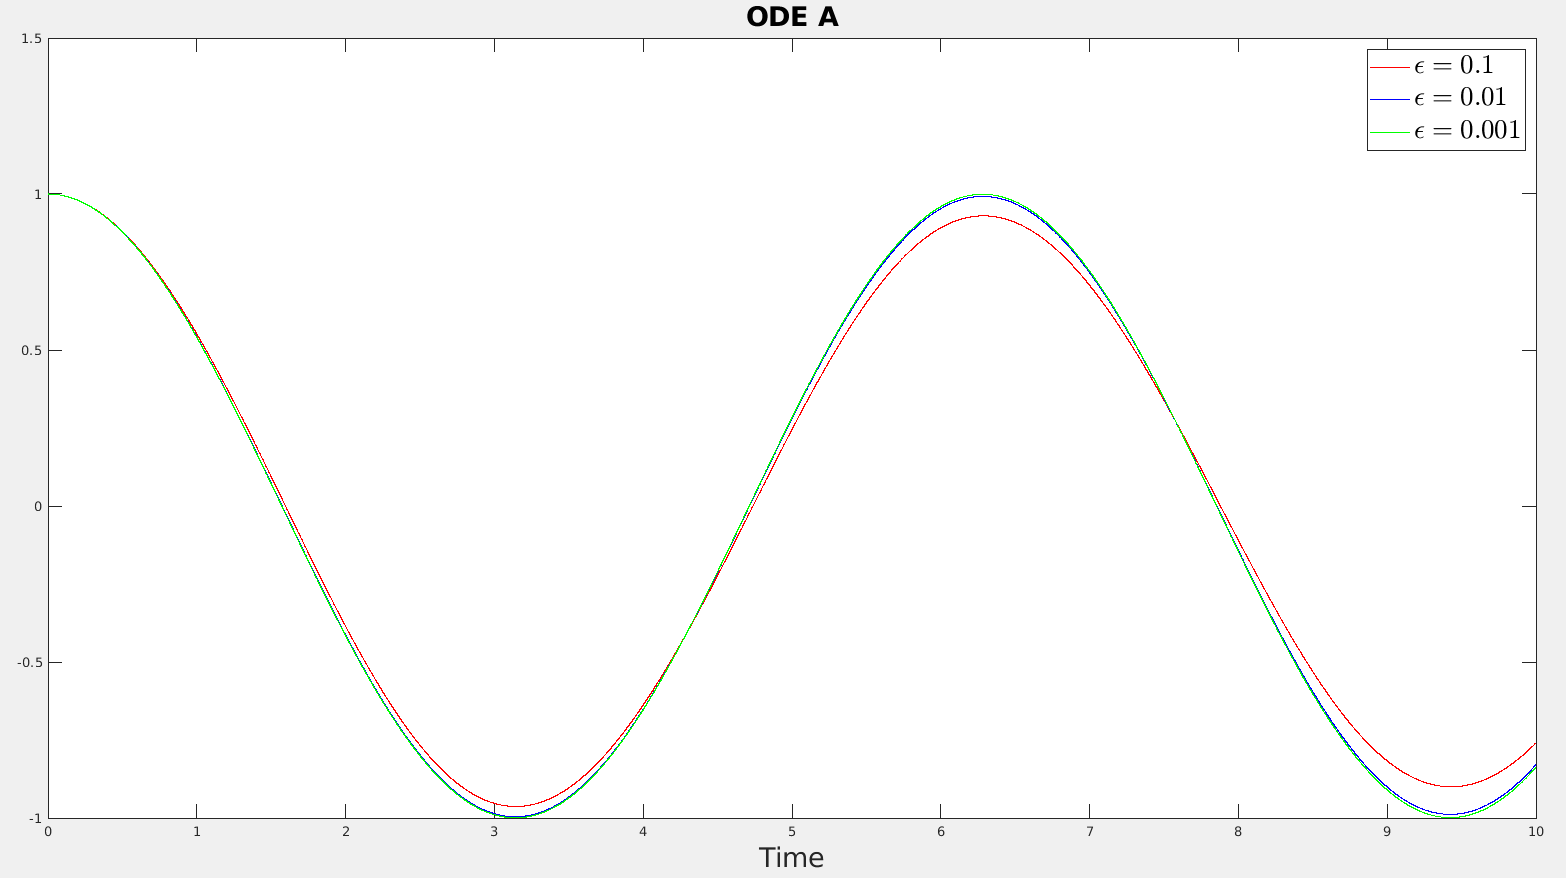
\includegraphics[width=\textwidth]{images/ODEA.png}
            \caption{Numerical Solution for differing $\epsilon$ using `ode45'}
            \label{fig:ODEA_num_sol}
        \end{figure}
    \item explanation
    \item lowest order uniformly converging solution
    \item Compare the numerical and analytical solutions for $\epsilon = 0.01$. 
\end{enumerate}

\vspace{20pt}

ODE B: 

\begin{gather*}
    \frac{d^2f}{dt^2} = -f - \epsilon f \left(\frac{df}{dt}\right)^4 \quad
    \text{with } f(0) = 1, \frac{df}{dt}(0) = 0
\end{gather*}

\begin{enumerate}[label=\alph*.]
    \item See Figure \ref{fig:ODEB_num_sol}
        \begin{figure}[ht]
            \centering
            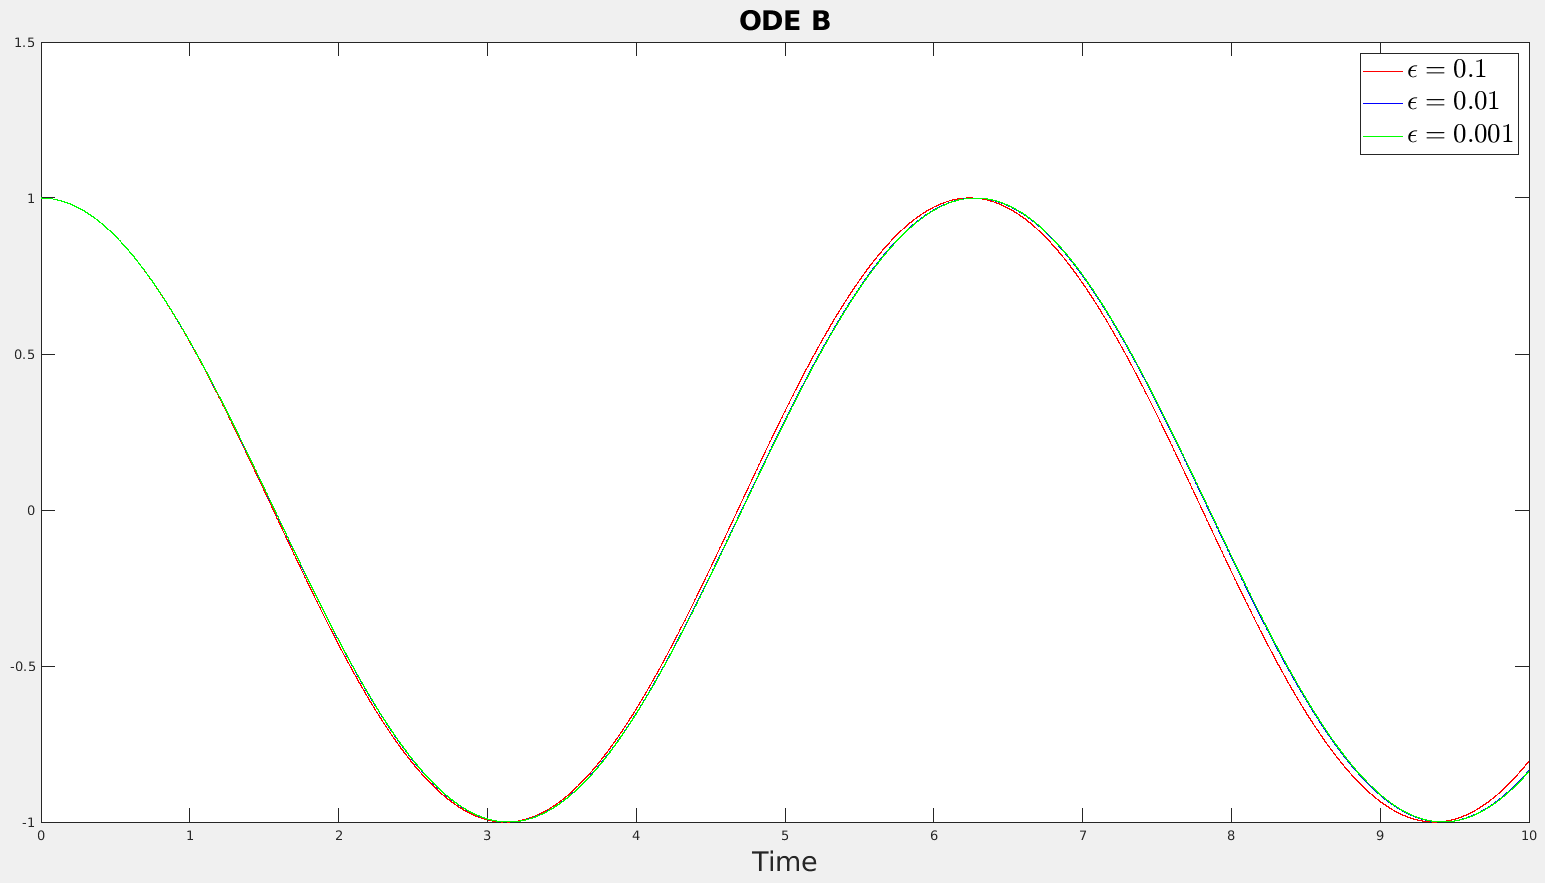
\includegraphics[width=\textwidth]{images/ODEB.png}
            \caption{Numerical Solution for differing $\epsilon$ using `ode45'}
            \label{fig:ODEB_num_sol}
        \end{figure}

    \item explanation
    \item lowest order uniformly converging solution
    \item Compare the numerical and analytical solutions for $\epsilon = 0.01$. 
\end{enumerate}

\vspace{20pt}

ODE C: 

\begin{gather*}
    \epsilon\frac{d^2f}{dt^2} + \frac{df}{dt} + (t+1)f = 0 \quad
    \text{with } f(0) = 1, f(1) = 2
\end{gather*}

\begin{enumerate}[label=\alph*.]
    \item See Figure \ref{fig:ODEC_num_sol}
        \begin{figure}[ht]
            \centering
            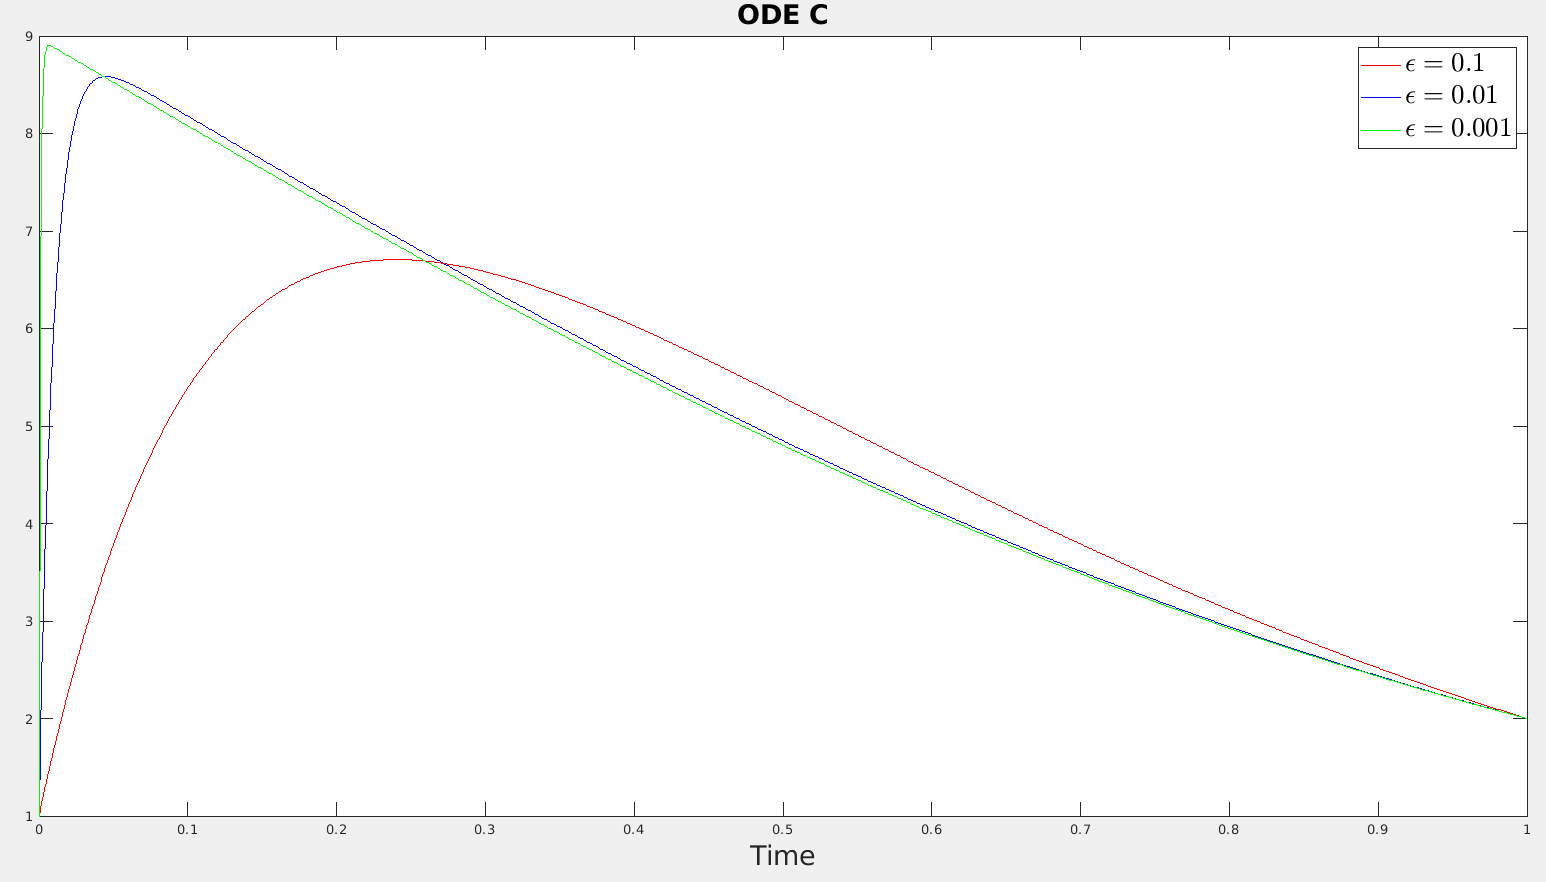
\includegraphics[width=\textwidth]{images/ODEC.png}
            \caption{Numerical Solution for differing $\epsilon$ obtained using
            the shooting method and `ode45'}
            \label{fig:ODEC_num_sol}
        \end{figure}
    \item explanation
    \item lowest order uniformly converging solution
    \item Compare the numerical and analytical solutions for $\epsilon = 0.01$. 
\end{enumerate}

\vspace{10pt}

\hline

\vspace{10pt}

\section*{Problem 2}
Find the eigenvalues and eigenfunctions of this eigenvalue problem, in the
limite where the eigenvalue $\lambda$ is very large and positive. 

\begin{gather*}
    \frac{d^2f}{dt^2} + \lambda(x+1)^2f = 0 \quad \text{with } f(1) = 0, f(2) =
    0
\end{gather*}

\end{document}


